% This file was created by tikzplotlib v0.9.2.
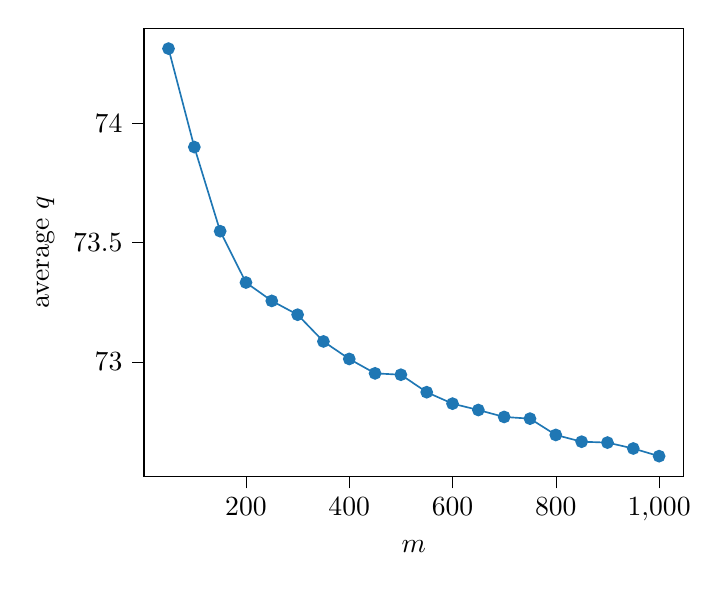
\begin{tikzpicture}

\definecolor{color0}{rgb}{0.12156862745098,0.466666666666667,0.705882352941177}
\definecolor{color1}{rgb}{0.976470588235294,0.450980392156863,0.0235294117647059}

\begin{axis}[
tick align=outside,
tick pos=left,
xlabel = $m$,
ylabel = average $q$,
x grid style={white!69.0196078431373!black},
xmin=2.5, xmax=1047.5,
xtick style={color=black},
y grid style={white!69.0196078431373!black},
%´ymin=72, ymax=91,
ymin=72.5198618350407, ymax=74.3989386078973,
ytick style={color=black},
scatter/classes={a={mark=o,draw=black}}
]
\addplot[scatter, scatter src=explicit symbolic, semithick, color0]
table {%
50 74.3135260273129
100 73.9007987162947
150 73.548228008839
200 73.3330687122862
250 73.256039993344
300 73.1981969846523
350 73.0861031936403
400 73.0127258791942
450 72.9523915686429
500 72.9466183308799
550 72.873379839116
600 72.8254219384188
650 72.7987235551989
700 72.7696569674668
750 72.7625372033231
800 72.6942015413158
850 72.6658903806182
900 72.6621935833012
950 72.6374432276665
1000 72.6052744156251
};

\end{axis}

\end{tikzpicture}
